\documentclass[12pt]{article}
 
\usepackage[margin=1in]{geometry} 
\usepackage{amsmath,amsthm,amssymb,amsfonts}
\usepackage{color}
\usepackage{graphicx}
\graphicspath{ {Images/} }
\usepackage{float}
\setlength{\parskip}{1em}
\usepackage{cancel}
\usepackage{longtable}
\usepackage{algorithm}
\usepackage{algpseudocode}
\usepackage{pgf,tikz,pgfplots}
\pgfplotsset{compat=1.15}
\usepackage{mathrsfs}
\usetikzlibrary{arrows}
\pagestyle{empty}
\begin{document}
	
	
\section*{Problem 2}

The following is the separable unconstrained optimisation problem to be solved:
\begin{align*}
\min_{x,y,z}\qquad& f_1(x,z)+f_2(y,z),
\end{align*}

where $x\in\mathbb{R}^n$, $y\in\mathbb{R}^m$, $z\in\mathbb{R}$ and $f_1$ and $f_2$ are quadratic in $n+1$ and $m+1$ variables respectively. In other words, the function $f_1$ has the form $f_1=\sum\limits_{i=1}^n \sum\limits_{j=i}^n a_{ij}x_ix_j + \sum\limits_{i=1}^n b_ix_i+c+\sum\limits_{i=1}^n d_izx_i+ez+fz^2$, for some coefficients $a_{ij},b_i,c,d_i,e,f$. The function $f_2$ can be similarly defined, $f_2=\sum\limits_{i=1}^m \sum\limits_{j=i}^m p_{ij}x_ix_j + \sum\limits_{i=1}^m q_ix_i+r+\sum\limits_{i=1}^m s_izx_i+tz+uz^2$, for some coefficients $p_{ij},q_i,r,s_i,t,u$.

Once again, $z$ is a shared variable that can be accessed by all agents, while $x$ and $y$ are both vectors of private variables that can only be accessed by Agent 1 and Agent 2 respectively.

By applying a change of variables, the cost function can be separated and the new formulation of the problem will be
\begin{align*}
\min_{x,\xi_1,y,\xi_2}\qquad& f_1(x,\xi_1)+f_2(y,\xi_2)\\
s.t.\qquad&\xi_1=\xi_2.
\end{align*}
The dual function will then be
\begin{align*}
q(\lambda)&=q_1(\lambda)+q_2(\lambda)\\
&=\inf_{x,\xi_1}[f_1(x,\xi_1)-\lambda\xi_1]+\inf_{y,\xi_2}[f_2(y,\xi_2)+\lambda\xi_2].
\end{align*}
The minimisers can be found by finding the gradients and setting to zero, as follows:
\begin{align*}
\nabla [f_1(x,\xi_1)-\lambda\xi_1]&=\begin{bmatrix}2a_{11}x_1+\sum\limits_{i\neq1} a_{1i}x_i+b_1+d_1\xi_1\\ \vdots\\ 2a_{nn}x_n+\sum\limits_{i\neq n} a_{ni}x_n+b_n+d_n\xi_1\\2f\xi_1+(e-\lambda)+\sum\limits_{i=1}^n d_ix_i\end{bmatrix}\\
&=\underbrace{\begin{bmatrix}2a_{11}&...&&a_{1n}&d_1\\&& \vdots\\ a_{1n}&...&&2a_{nn}&d_n\\d_1&...&&d_n&2f\end{bmatrix}}_{A_1} \begin{bmatrix}x_1\\ \vdots\\ x_n\\\xi_1\end{bmatrix}+\underbrace{\begin{bmatrix}b_1\\ \vdots\\ b_n\\(e-\lambda)\end{bmatrix}}_{B_1}=\textbf{0}
\end{align*}
\begin{align*}
\nabla [f_2(y,\xi_2)+\lambda\xi_2]&=\begin{bmatrix}2u\xi_2+(t+\lambda)+\sum\limits_{i=1}^m s_iy_i\\2p_{11}y_1+\sum\limits_{i\neq1} p_{1i}y_i+q_1+s_1\xi_2\\ \vdots\\ 2p_{mm}x_m+\sum\limits_{i\neq m} q_{mi}y_m+q_m+s_m\xi_2\end{bmatrix}\\
&=\underbrace{\begin{bmatrix}2u&s_1&...&&s_m\\ s_1&2p_{11}&...&&p_{1m}\\&&\vdots\\ s_m&p_{1m}&...&&2p_{mm}\end{bmatrix}}_{A_1} \begin{bmatrix}\xi_2\\y_1\\ \vdots\\ y_m\end{bmatrix}+\underbrace{\begin{bmatrix}(t+\lambda)\\q_1\\ \vdots\\ q_m\end{bmatrix}}_{B_1}=\textbf{0}
\end{align*}
The minimiser of $[f_1(x,\xi_1)-\lambda\xi_1]$ is then the solution to the set of $n+1$ linear equations and the minimiser of $[f_2(y,\xi_2)+\lambda\xi_2]$ is the solution to the set of $m+1$ linear equations above. Note, the matrices $A_1$  and $A_2$ are symmetric and must be invertible, i.e., their eigenvalues must be strictly positive; the problem is ill-conditioned if the eigenvalues are close to zero.

The same method of using the subgradient and dual decomposition from Problem 1 now applies to this problem.

\subsection*{Combined Problem}
At this stage it is useful to observe the problem without separation, where the cost function is optimised as a single function. The problem is quadratic, and the minimiser is found by solving $n+m+1$ linear equations. This means solving the problem $Ax=B$, with $A$ and $B$ found by augmenting and overlapping $A_1,A_2$ and $B_1,B_2$ respectively. This is visualised below.

\begin{figure}[H]
	\centering
	\definecolor{rvwvcq}{rgb}{0.08,0.4,0.7}
	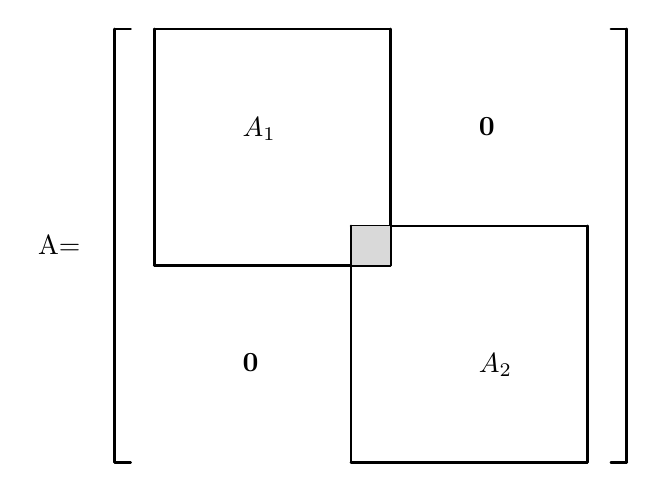
\begin{tikzpicture}[line cap=round,line join=round,>=triangle 45,x=1cm,y=1cm]
	\draw [line width=1pt] (9.5,10)-- (9.5,4.5);
	\draw [line width=1pt] (9.5,10)-- (9.7,10);
	\draw [line width=1pt] (9.7,4.5)-- (9.5,4.5);
	\draw [line width=1pt] (16,10)-- (16,4.5);
	\draw [line width=1pt] (15.8,10)-- (16,10);
	\draw [line width=1pt] (15.8,4.5)-- (16,4.5);
	\draw [line width=1pt] (10,10)-- (10,7);
	\draw [line width=1pt] (10,7)-- (13,7);
	\draw [line width=1pt] (13,7)-- (13,10);
	\draw [line width=1pt] (13,10)-- (10,10);
	\draw [line width=1pt] (12.5,7.5)-- (12.5,4.5);
	\draw [line width=1pt] (12.5,4.5)-- (15.5,4.5);
	\draw [line width=1pt] (15.5,4.5)-- (15.5,7.5);
	\draw [line width=1pt] (15.5,7.5)-- (12.5,7.5);
	\draw[fill=gray!30]    (13,7) -- (13,7.5) -- (12.5,7.5) -- (12.5,7);
	\draw (11,9) node[anchor=north west] {$A_1$};
	\draw (14,6) node[anchor=north west] {$A_2$};
	\draw (11,6) node[anchor=north west] {\textbf{0}};
	\draw (14,9) node[anchor=north west] {\textbf{0}};
	\draw (8.4,7.5) node[anchor=north west] {A=};
	\end{tikzpicture}
	\caption{Overlapping squares represent how $A_1$ and $A_2$ overlap. There is a single element in the grey overlapping region and it is equal to $2f+2u$, the sum of the elements of $A_1$ and $A_2$ that overlap.}
\end{figure}

\begin{figure}[H]
	\centering
	\definecolor{rvwvcq}{rgb}{0.08,0.4,0.7}
	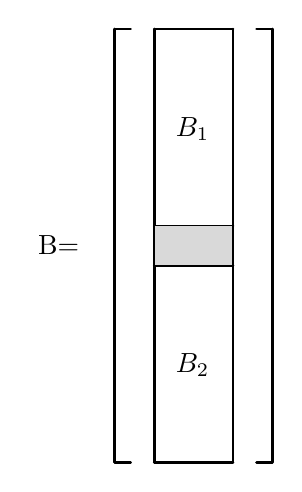
\begin{tikzpicture}[line cap=round,line join=round,>=triangle 45,x=1cm,y=1cm]
	\draw [line width=1pt] (9.5,10)-- (9.5,4.5);
	\draw [line width=1pt] (9.5,10)-- (9.7,10);
	\draw [line width=1pt] (9.7,4.5)-- (9.5,4.5);
	\draw [line width=1pt] (11.5,10)-- (11.5,4.5);
	\draw [line width=1pt] (11.3,10)-- (11.5,10);
	\draw [line width=1pt] (11.3,4.5)-- (11.5,4.5);
	\draw [line width=1pt] (10,10)-- (10,7);
	\draw [line width=1pt] (10,7)-- (11,7);
	\draw [line width=1pt] (11,7)-- (11,10);
	\draw [line width=1pt] (11,10)-- (10,10);
	\draw [line width=1pt] (10,7.5)-- (10,4.5);
	\draw [line width=1pt] (10,4.5)-- (11,4.5);
	\draw [line width=1pt] (11,4.5)-- (11,7.5);
	\draw [line width=1pt] (11,7.5)-- (10,7.5);
	\draw[fill=gray!30]    (11,7) -- (11,7.5) -- (10,7.5) -- (10,7);
	\draw (10.15,9) node[anchor=north west] {$B_1$};
	\draw (10.15,6) node[anchor=north west] {$B_2$};
	\draw (8.4,7.5) node[anchor=north west] {B=};
	\end{tikzpicture}
	\caption{Similarly, $B$ is a vector with $B_1$ and $B_2$ overlapping as shown. Only one element is in the grey overlapping region, and that element is equal to $e+t$, the sum of the elements of $B_1$ and $B_2$ that overlap.}
\end{figure}
We can solve the combined problem and use it to check the convergence of the decomposed problem.

\subsection*{Convergence}
As a reminder, in separating the cost function, it is now a requirement that both $A_1$ and $A_2$ are well-conditioned in order to get convergence. The combined matrix $A$ may be well conditioned, but depending on how $A_1$ and $A_2$ are separated, we may end up with an ill-conditioned matrices.

This picks up from where Problem 1 left off. In Problem 1, convergence was still guaranteed regardless of how the shared variable $x_3^2$ was separated. It turns out that this does not hold for coefficients of $x_3^2$ that are too close to zero. If the coefficient of $x_3^2$ is too small, convergence no longer occurs. Thus, we see the key requirement that the matrices are well-conditioned appearing in Problem 1 as well.

When the problem is well-conditioned, the separated problem when the dual decomposition with subgradient method is used converges to the solution obtained by solving the combined problem.

\begin{figure}[H]
	\includegraphics[scale=1]{Problem2-Convergence.png}
\end{figure}

\subsection*{Computational Overhead}

There is some computational overhead to spawn a Process on Python. Previously in Problem 1, a dummy for-loop was added to increase the complexity of each parallel process. For Problem 2, we achieve the same affect by increasing $n$ and $m$, i.e., increasing the dimensions of $A_1$ and $A_2$. The following plot shows the completion times, where the dimensions of $A_1$ and $A_2$ have been set to be equal.

\begin{figure}[H]
	\includegraphics[scale=1]{Problem2-TimeTrial.png}
\end{figure}

In Problem 1, the increase in completion times for both serial and parallel were linear. This was because a single dummy for-loop was used to simulate increasing the complexity of the processes. In Problem 2, the solution to $A_1x+B_1$ and $A_2x+B_2$ were found by applying Gaussian elemination, which has a complexity of order $\mathcal{O}(n^3)$. The sample plot above may not be enough to conclude cubic growth as the dimensions of the problem grow, but it can be seen that the growth is of order higher than linear growth.


\subsection*{How to Run}

\subsubsection*{The above examples}

Make sure you are in the correct directory. Then to run the test that generated the above plots, execute the \textbf{main.py} file, i.e. use the command

\noindent \textbf{$>>>$python main.py}

\subsubsection*{Function Descriptions}

The function \textbf{parallel.do\_parallel}, description.

Syntax: do\_parallel(max\_iter,alpha,A1,A2,b1,b2,verbose=False)

Parameter values:
\begin{itemize}
	\item max\_iter, Required. Number of iterations for the subgradient method.
	\item alpha, Required. Step size for the subgradient method.
	\item A1, Required. The matrix of coefficients $A_1$ as described above.
	\item A2, Required. The matrix of coefficients $A_2$ as described above.
	\item b1, Required. The matrix of coefficients $B_1$ as described above.
	\item b2, Required. The matrix of coefficients $B_2$ as described above.
	\item verbose, Default False. Print results to screen.
\end{itemize}

Outputs:
\begin{itemize}
	\item Output 1. List containing $\xi_1^*$ for all iterations of the subgradient method.
	\item Output 2. List containing $\xi_2^*$ for all iterations of the subgradient method.
	\item Output 3. Completion time.
\end{itemize}

\end{document}